\documentclass{article}
\usepackage[utf8]{inputenc}
\usepackage{graphicx}
\usepackage{hyperref}
\usepackage{amsmath}
\usepackage{booktabs}
\usepackage{float}
\usepackage{geometry}
\usepackage{xcolor}
\usepackage{titlesec}
\usepackage{enumitem}
\usepackage{fontspec}
\usepackage{microtype}
\usepackage{fancyhdr}
\usepackage{lastpage}

% Modern geometry settings
\geometry{a4paper, margin=1in}

% Modern colors
\definecolor{maincolor}{RGB}{41, 128, 185}
\definecolor{secondcolor}{RGB}{52, 73, 94}
\definecolor{accentcolor}{RGB}{231, 76, 60}

% Modern section formatting
\titleformat{\section}
  {\normalfont\Large\bfseries\color{maincolor}}
  {\thesection}{1em}{}[\titlerule]
  
\titleformat{\subsection}
  {\normalfont\large\bfseries\color{secondcolor}}
  {\thesubsection}{1em}{}

% Modern list formatting
\setlist[itemize]{leftmargin=*,label=\textcolor{maincolor}{$\bullet$}}

% Modern header/footer
\pagestyle{fancy}
\fancyhf{}
\fancyhead[L]{\textcolor{secondcolor}{Cat Breed Classification}}
\fancyhead[R]{\textcolor{secondcolor}{Page \thepage\ of \pageref{LastPage}}}
\fancyfoot[C]{\textcolor{secondcolor}{PyTorch Capstone Project}}
\renewcommand{\headrulewidth}{0.4pt}
\renewcommand{\footrulewidth}{0.4pt}

% Hyperref settings
\hypersetup{
    colorlinks=true,
    linkcolor=maincolor,
    filecolor=maincolor,      
    urlcolor=accentcolor,
    citecolor=maincolor,
}

\title{\textcolor{maincolor}{\Huge PyTorch Capstone Project Report}\\
\textcolor{secondcolor}{\Large Cat Breed Classification System}}
\author{\textcolor{secondcolor}{Wiwat Pholsomboon}}

\date{\textcolor{secondcolor}{April 8, 2025}}

\begin{document}

\maketitle

\section{Introduction}
This project is to study on using PyTorch model to classify cat images. It implements Grad-CAM to visualized the attention of the model on one of CNN layers. ChatGPT-4o-mini is integrated to classify cat images and given the rationale of its result. Quiz is implemented to show the accuracy of each model along with human accuracy.

Github: \href{https://github.com/innozent/pytorch_capstone}{https://github.com/innozent/pytorch\_capstone}

\section{Dataset}
\begin{itemize}
    \item Dataset is from Kaggle from 'Geno Cat Breed Image Collection' dataset (\url{https://www.kaggle.com/datasets/shawngano/gano-cat-breed-image-collection})
    \item Contains 15 cat breeds with 375 photos for each breed (total 5,625 photos)
    \item Preprocessing step
    \begin{itemize}
        \item Resize to 256x256
        \item Random Crop to 224x224
        \item Random Horizontal Flip
        \item Random Rotation
        \item Convert to Tensor
        \item Normalize with mean and std of ImageNet
    \end{itemize}
\end{itemize}

\section{Model Architecture}
\begin{itemize}
    \item Architecture of implemented models:
    \begin{itemize}
        \item 5 Convolutional Layers (Conv2d)
        \item 2 Fully Connected Layers (Linear)
        \item 1 Dropout Layer (Dropout)
        \item ReLU Activation Function
    \end{itemize}
    \item Transfer Learning Models:
    \begin{itemize}
        \item ResNet18 Model (Weights: ImageNet)
        \item EfficientNetB2 Model (Weights: ImageNet)
        \item VGG16 Model (Weights: ImageNet)
    \end{itemize}
    \item GPT Model:
    \begin{itemize}
        \item ChatGPT-4o-mini implemented from OpenRouter API
        \item Evaluate the model accuracy use quiz.
    \end{itemize}
\end{itemize}

\section{Training Methodology}
\begin{itemize}
    \item All models are trained with the same hyperparameters for fair comparison.
    \begin{itemize}
        \item Training Batch Size: 128
        \item Learning Rate: 0.001
        \item Momentum: 0.9
        \item Epochs: 5
        \item Loss Function: Cross Entropy Loss
        \item Optimizer: SGD
    \end{itemize}
\end{itemize}

\section{Results and Evaluation}
\begin{itemize}
    \item Compare Training Accuracy and Loss of each model.
    \item Quiz is implemented to show the accuracy of each model along with human accuracy and ChatGPT-4o-mini accuracy.
\end{itemize}


\begin{figure}[H]
    \centering
    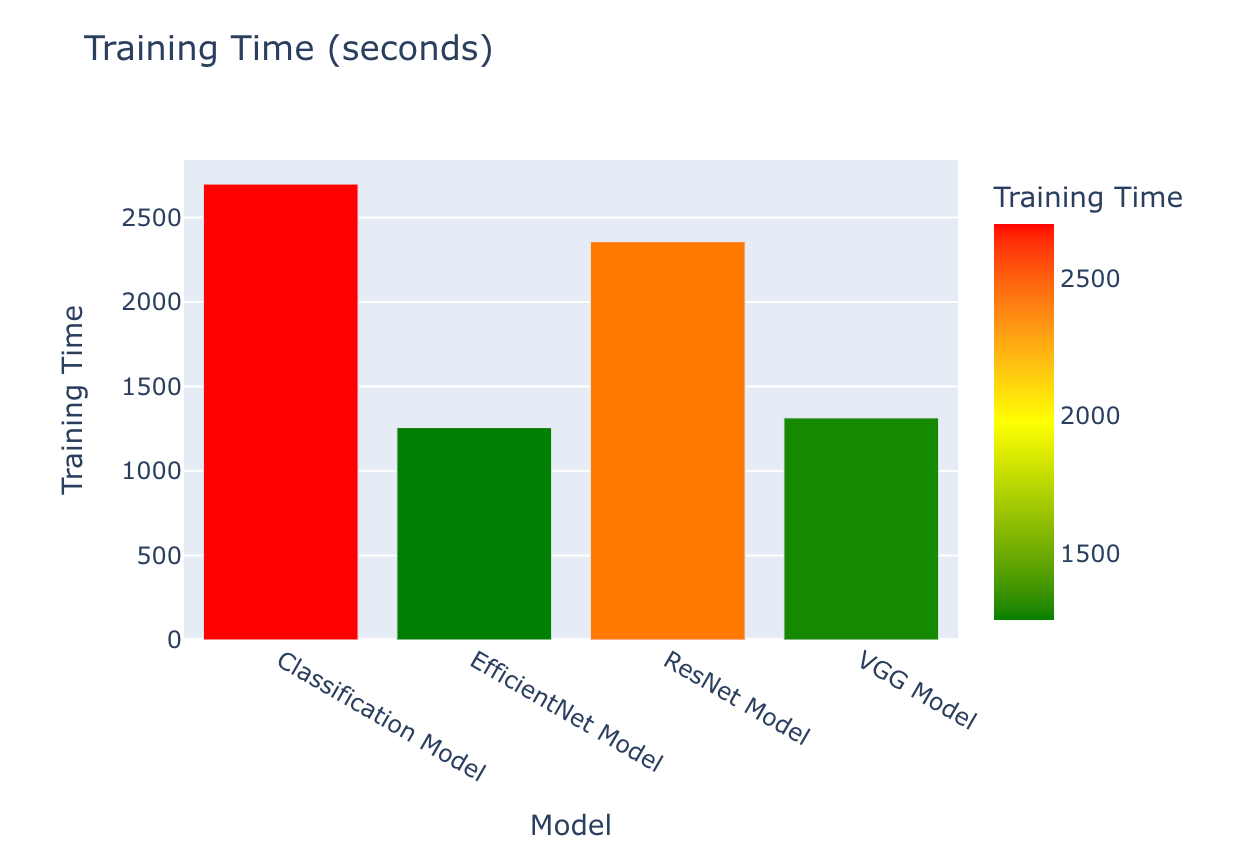
\includegraphics[width=0.80\textwidth]{eval4.png} 
    \caption{Comparison of training time}
    \label{fig:training_time}
\end{figure}

\begin{figure}[H]
    \centering
    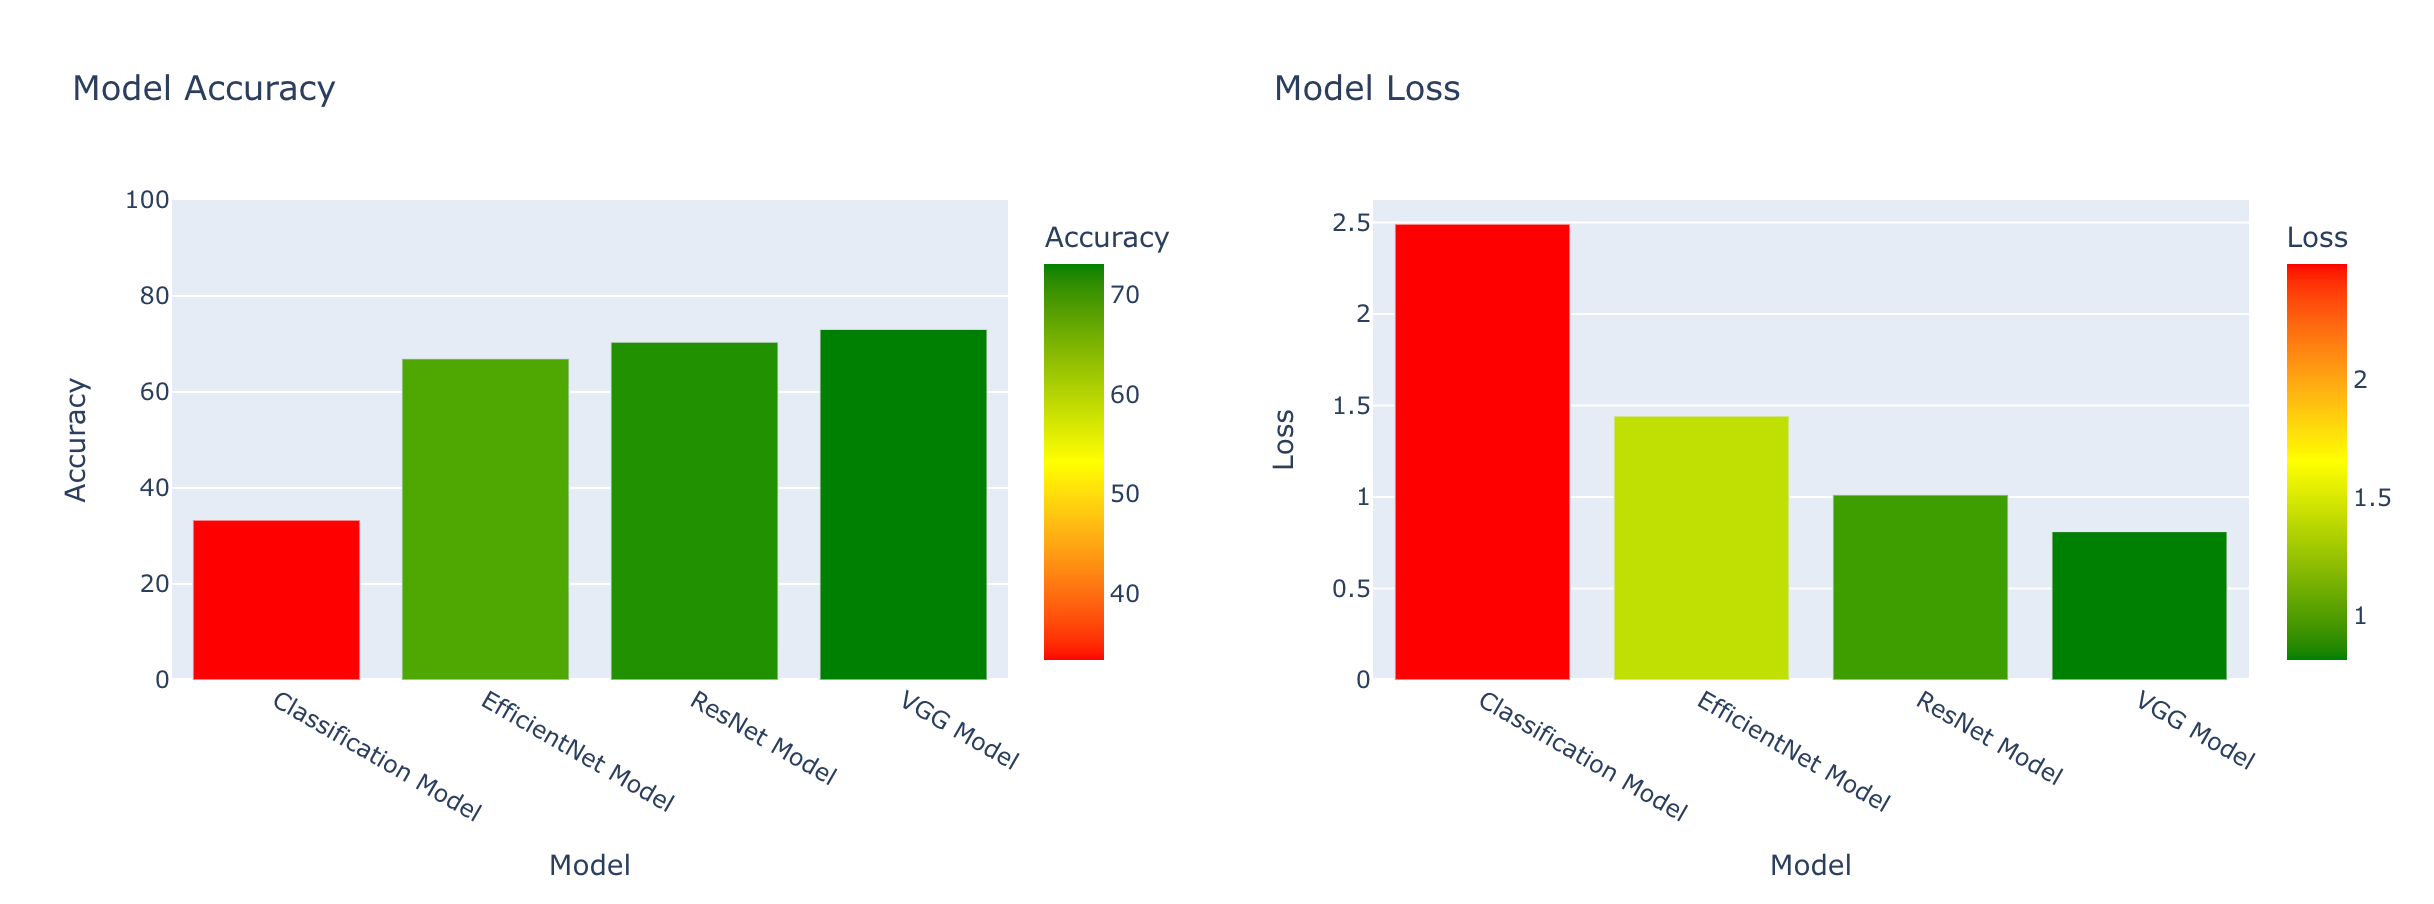
\includegraphics[width=\textwidth]{eval1.png}
    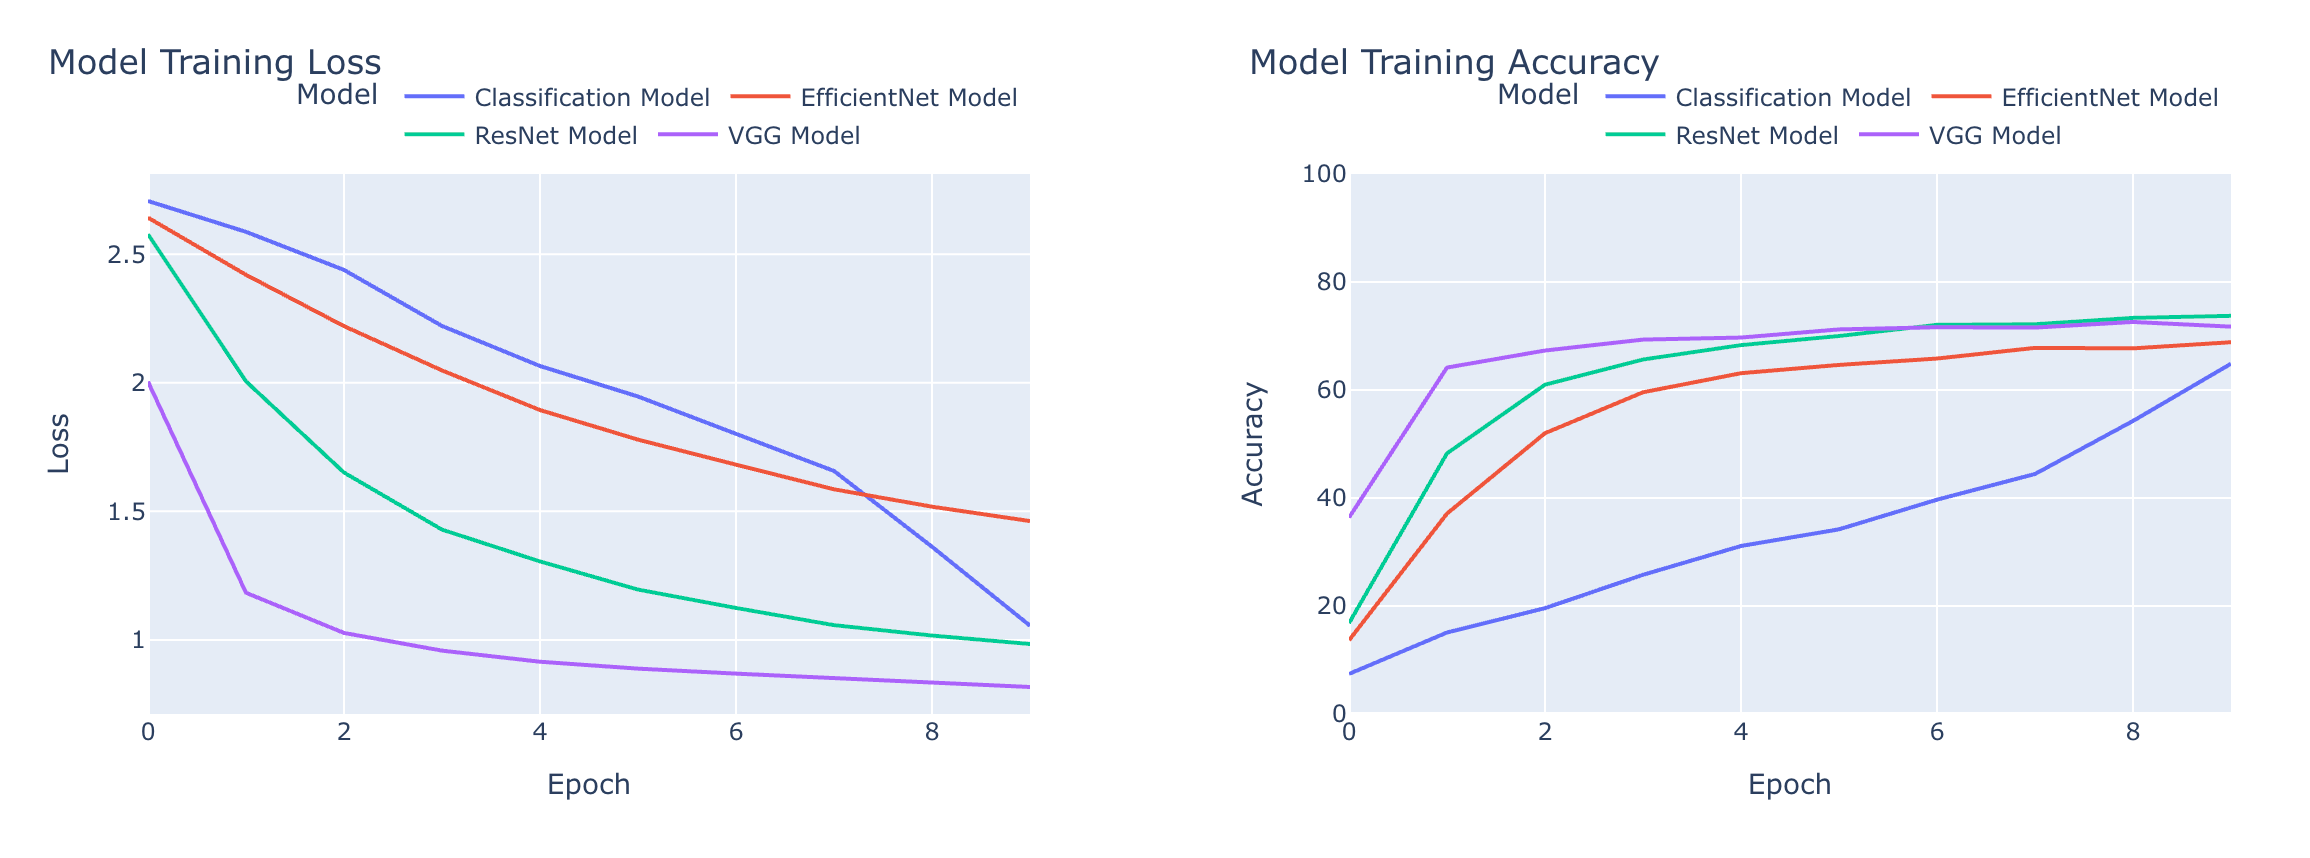
\includegraphics[width=\textwidth]{eval2.png}
    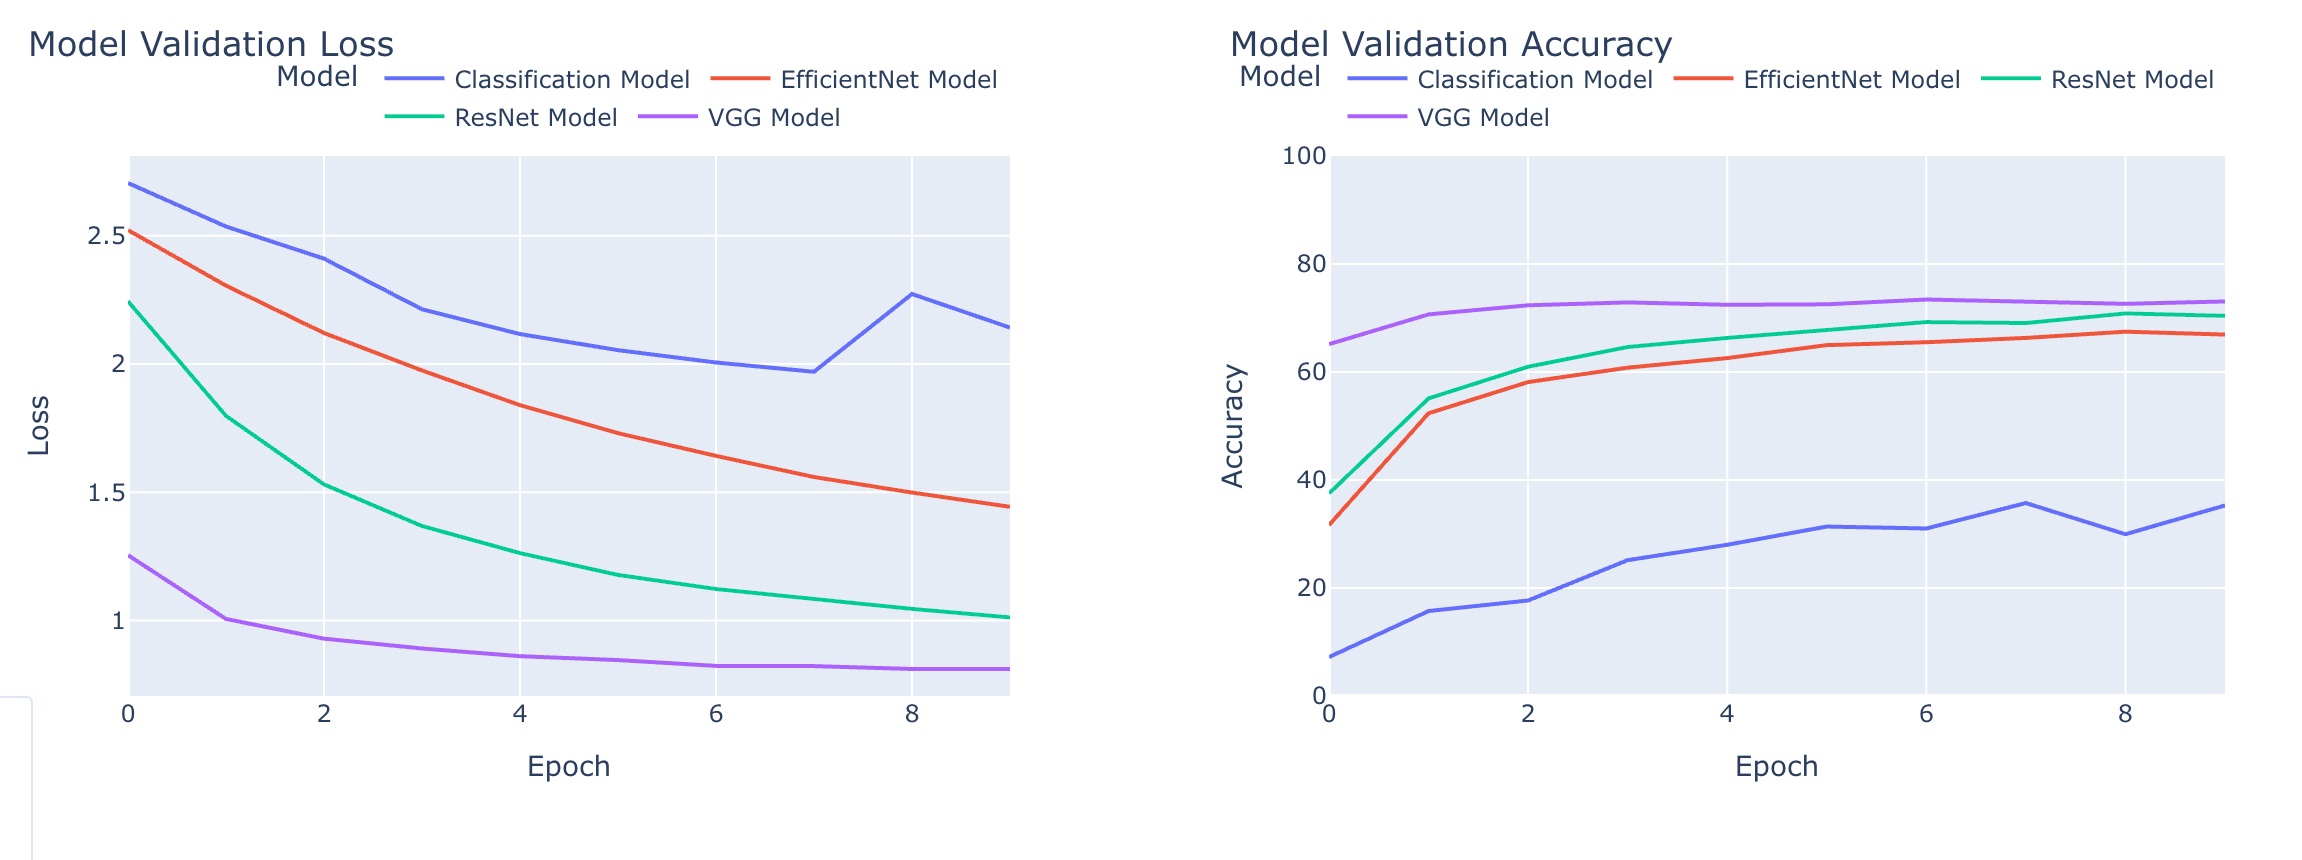
\includegraphics[width=\textwidth]{eval3.png}
    \caption{Comparison of model accuracy and loss}
    \label{fig:models}
\end{figure}


\section{Visualization and Interpretability}
\begin{itemize}
    \item Implemented Grad-CAM to compared and visualize each model's attention on the image
    \item ChatGPT-4o-mini will give the rationale of its answer.
\end{itemize}

\begin{figure}[H]
    \centering
    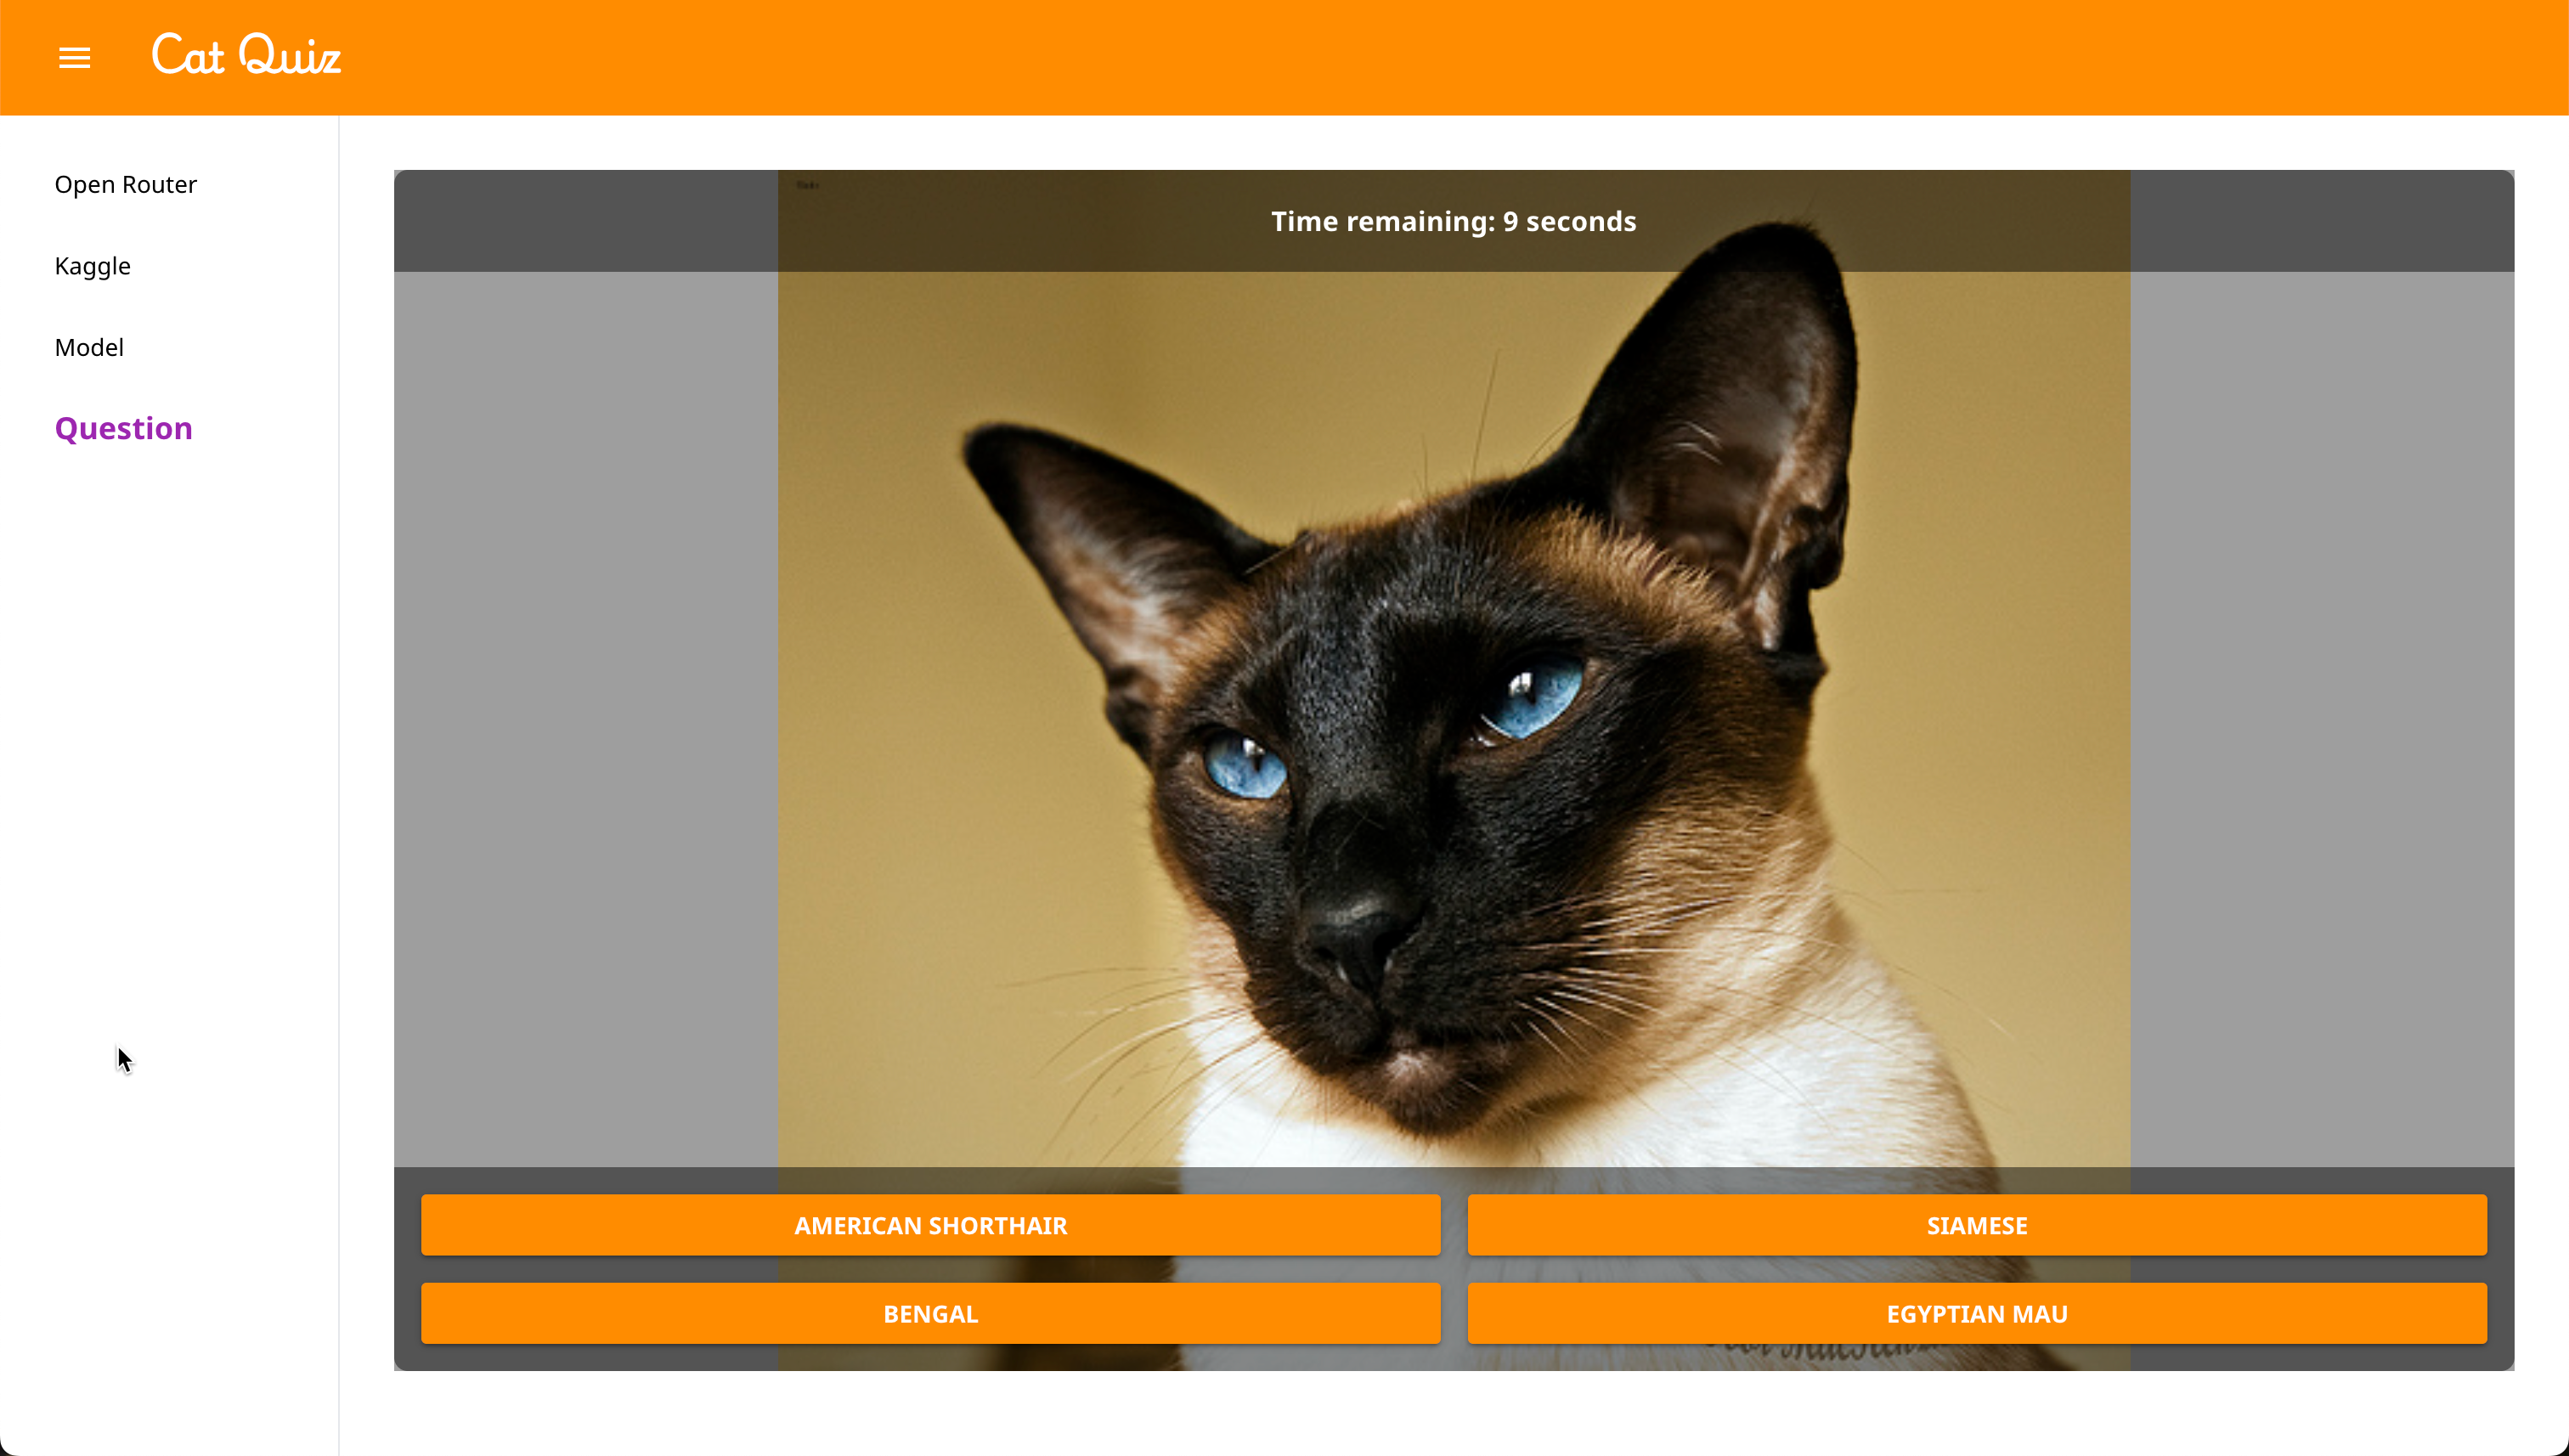
\includegraphics[width=\textwidth]{quiz.png}
    \caption{Quiz interface allow user to choose the answers}
    \label{fig:quiz}
\end{figure}


\begin{figure}[H]
    \centering
    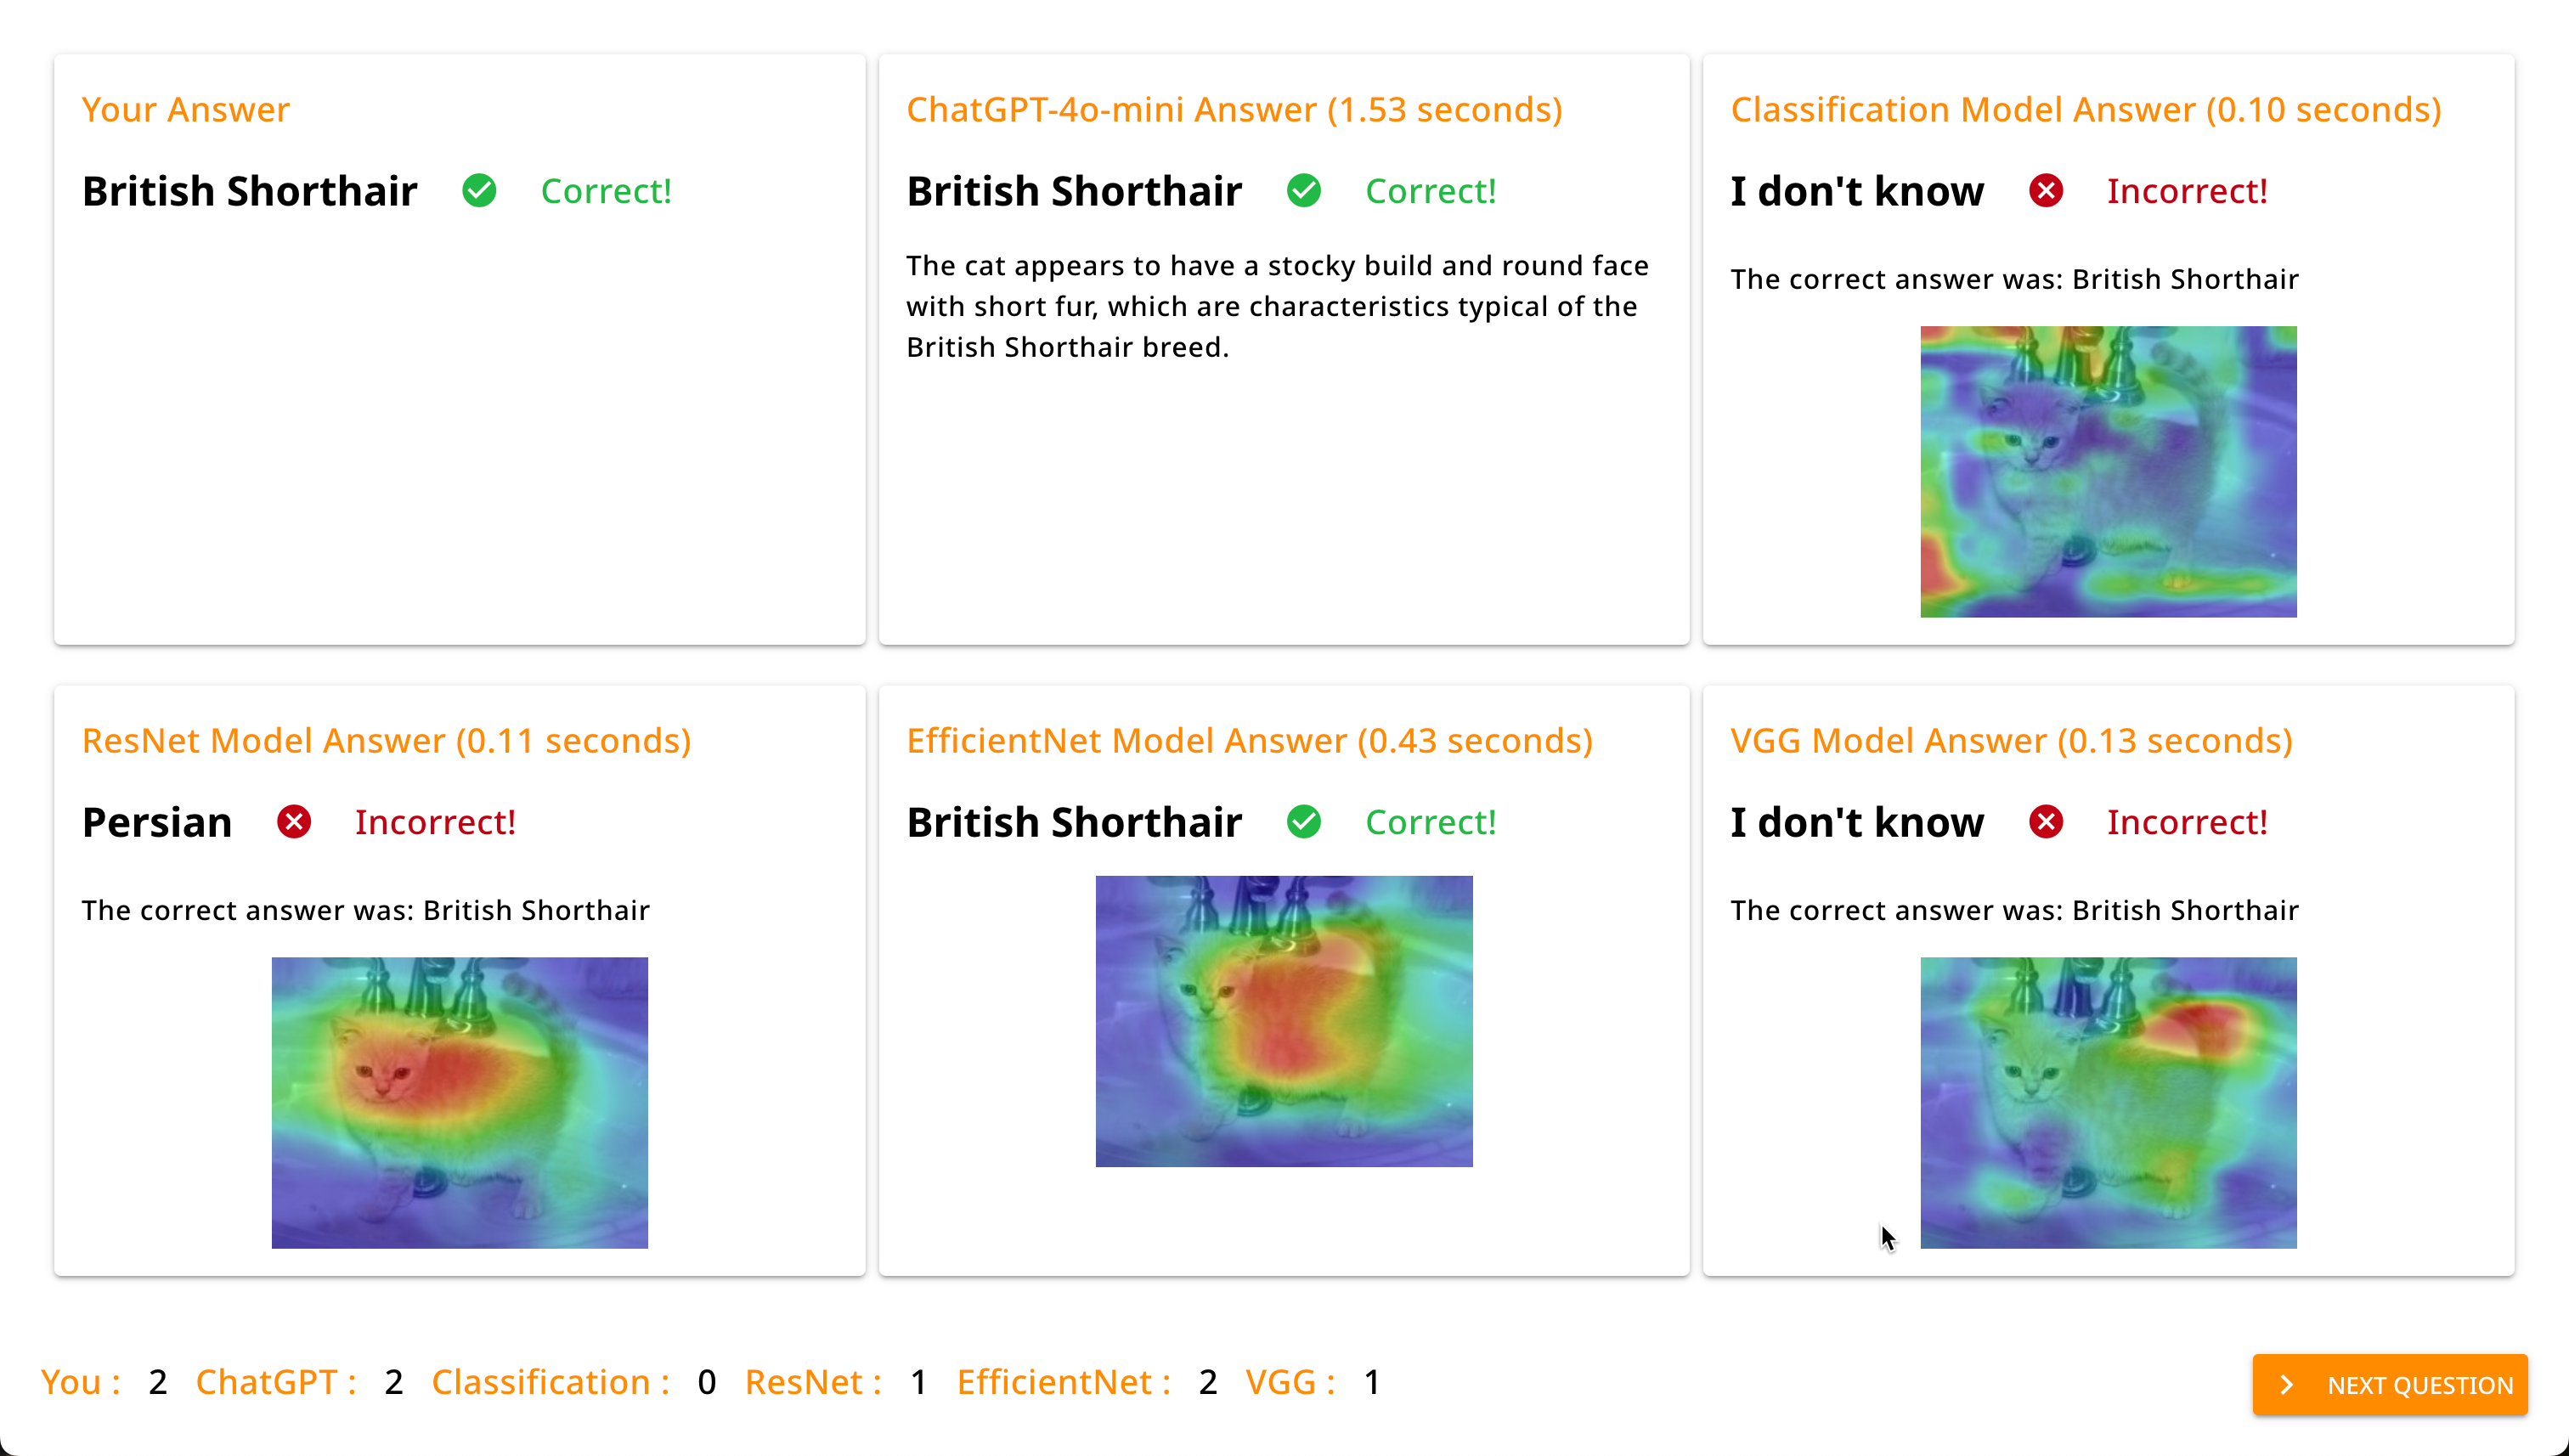
\includegraphics[width=\textwidth]{evaluation.png}
    \caption{Evaluation results comparing human, ChatGPT-4o-mini and PyTorch Models accuracy}
    \label{fig:evaluation}
\end{figure}

\section{Challenges and Solutions}
\begin{itemize}
    \item Grad-CAM target layer for each model architecture is different and need to be selected manually.
    \begin{itemize}
        \item Solution is to print out model architecture and select the CNN layer at very last stage of the model.
    \end{itemize} 
\end{itemize}

\section{Future Improvements}
\begin{itemize}
    \item Add users management to save the quiz result and compare with the previous quiz result.
    \item Add more data augmentation techniques.
    \item Add more models for comparison.
    \item Add more evaluation metrics.
\end{itemize}

\section{Conclusion}
\begin{table}[H]
    \centering
    \begin{tabular}{lrrrr}
    \toprule
    \textbf{Model} & \textbf{Parameters} & \textbf{Accuracy} & \textbf{Loss} & \textbf{Training Time (s)} \\
    \midrule
    Custom CNN Model & 31.9M & 42\% & 1.86 & 2,698 \\
    EfficientNet Model & 9.1M & 71\% & 1.40 & 1,256 \\
    ResNet Model & 11.7M & 73\% & 0.99 & 2,357 \\
    VGG Model & 138.3M & 76\% & 0.81 & 1,314 \\
    \bottomrule
    \end{tabular}
    \caption{Comparison of model performance metrics}
    \label{tab:model_comparison}
\end{table}

\begin{itemize}
    \item VGG16 Model is the best model based on confusion matrix and accuracy score, but it contains a very large number of parameters (138 Million parameters).
    \item ResNet18 Model, on the other hand, has a smaller number of parameters (11.7 Million parameters) and nearly the same performance as VGG16.
    \item EfficientNet B2 has 9.1 Million parameters and slightly lower accuracy compared to VGG16 and ResNet18 on this dataset.
    \item ChatGPT-4o-mini, which is a multi-modal model, has image recognition capabilities. It can be used for cat image classification and provides rationale for its predictions.
\end{itemize}

\end{document}
